%--------------------------------------------------------------------------
\chapter{APPLICATIONS AND CONCLUSION}

%TODO: add tests to confirm results

%--------------------------------------------------------------------------
\section{Single and multi-threaded command-line tools}

%--------------------------------------------------------------------------
This section exemplifies the use of the framework developed in the previous chapter by defining two command-line tools for computing combination matrices of self-derivation. The first of them computes all solutions for a given row and problem size using a single thread of execution, while the second utilizes several threads. The single-threaded application is reasonably fast for small row and problem sizes. As input sizes grow, the number of solutions grows dramatically, and a single thread of execution becomes insufficient.

%--------------------------------------------------------------------------
\begin{lstlisting}[caption={A single-threaded command line tool.},label={singleMain}]
int main(int argc, char *argv[]) {
    if (argc < 3) {
        printf("Enter a problem size and a row!\n");
        return -1;
    }

    common_data commonData;
    createCommonData(&commonData, argc, argv);

    thread_data data;
    createThreadData(&data, &commonData);

    clock_t start = clock();
    writeSolutions(&data, &commonData, 0, commonData.numTops);

    printf("%f seconds elapsed.\n", ((double) (clock() - start)) / CLOCKS_PER_SEC);
    printf("%lu solutions found!\n", data.counter);

    destroyThreadData(&data);
    destroyCommonData(&commonData);

    return 0;
}
\end{lstlisting}

%--------------------------------------------------------------------------
\begin{enumerate}
\item The inputs are the standard command line inputs, that is, the number of arguments, and the array of strings containing them.
\item Line 2 checks that at least three arguments were passed and, if not, line 3 prints usage instructions to the console and line 4 returns an error.
\addtocounter{enumi}{4}
\item Line 7 creates an empty thread-common data structure and line 8 calls Listing~\ref{createCommonData} to fill it.
\addtocounter{enumi}{2}
\item Line 10 creates an empty thread-specific data structure and line 11 calls Listing~\ref{createThreadData} to fill it.
\addtocounter{enumi}{2}
\item Line 13 computes the current time and stores it in a variable. Line 14 calls Listing~\ref{writeSolutions} to write solutions for all tops to a single text file.
\addtocounter{enumi}{2}
\item Line 16 computes the current time after the call to Listing~\ref{writeSolutions} in line 14, subtracts from it the start time computed in line 13, converts the result to seconds and prints it to the console. Line 17 prints to the console the number of solutions found.
\addtocounter{enumi}{2}
\item Lines 19 and 20 free all allocated memory by calling respectively Listing~\ref{destroyThreadData} and Listing~\ref{destroyCommonData}.
\addtocounter{enumi}{2}
\item Line 22 simply exits the program normally.
\end{enumerate}

%TODO: add table with execution times

%--------------------------------------------------------------------------
Listing~\ref{thread_manager} below describes a data structure that is used in Listing~\ref{multiMain} to manage multiple threads of execution. The framework described in the previous chapter was designed using only platform-independent components of the C programming language. For multi-threaded applications, the C programming language does not provide such platform-independent components. Listing~\ref{multiMain} therefore is written in C++, which provides a standard library for managing threads in a platform-independent way, as well as an object-oriented paradigm in which the creation, dispatching, and destruction of threads can be greatly simplified.

%--------------------------------------------------------------------------
\begin{lstlisting}[caption={A class to manage concurrency.},label={thread_manager}]
class thread_manager {
public:
    thread_manager(int argc, char *argv[]) : threadData(std::thread::hardware_concurrency()) {
        createCommonData(&commonData, argc, argv);

        for (auto &data: threadData)
            createThreadData(&data, &commonData);
    }

    ~thread_manager() {
        for (auto &data: threadData)
            destroyThreadData(&data);

        destroyCommonData(&commonData);
    }

    long long runThreads() {
        auto numThreads = threadData.size();

        auto doWork = [this, &numThreads](int i, length startTop, length endTop) {
            writeSolutions(&threadData[i], &commonData, startTop, endTop);
            std::lock_guard<std::mutex> lock(mutex);
            numThreads--;
            condition.notify_one();
        };

        length startTop = 0;
        length offset = commonData.numTops / numThreads;
        auto maxThreads = numThreads - 1;
        auto startTime = std::chrono::high_resolution_clock::now();

        for (auto i = 0; i < maxThreads; ++i) {
            std::thread(doWork, i, startTop, startTop + offset).detach();
            startTop += offset;
        }

        doWork(maxThreads, startTop, commonData.numTops);

        std::unique_lock<std::mutex> lock(mutex);
        condition.wait(lock, [&numThreads] { return numThreads == 0; });

        auto stopTime = std::chrono::high_resolution_clock::now();
        auto duration = std::chrono::duration_cast<std::chrono::milliseconds>(stopTime - startTime);

        return duration.count();
    }

    length getNumSolutions() const {
        length numSolutions = 0;

        for (auto &data: threadData)
            numSolutions += data.counter;

        return numSolutions;
    }

private:
    std::vector<thread_data> threadData;
    common_data commonData;
    std::mutex mutex;
    std::condition_variable condition;
};
\end{lstlisting}

%--------------------------------------------------------------------------
\begin{enumerate}
\addtocounter{enumi}{2}
\item The constructor of a thread manager in line 3 takes as inputs the same arguments passed on the command line, initializing the vector of thread-specific data structures declared in line 57 with the number of hardware cores in the CPU. Using more threads than the number of CPU cores does not necessarily improve performance. Line 4 then allocates the thread-common data with a call to Listing~\ref{createCommonData}, storing it to the member variable declared in line 58.
\addtocounter{enumi}{2}
\item The for loop in line 6 iterates through the vector of thread-specific data structures and allocates memory for each one of them in line 7 with calls to Listing~\ref{createThreadData}.
\addtocounter{enumi}{4}
\item The destructor of a thread manager iterates through the vector of thread-specific data structures, freeing the memory allocated in line 12 for each one of them with calls to Listing~\ref{destroyThreadData}.
\addtocounter{enumi}{2}
\item Line 14 frees the allocated thread-specific data in the destructor of a thread manager with a call to Listing~\ref{destroyCommonData}.
\addtocounter{enumi}{2}
\item Line 17 declares the \emph{runThreads} method, which takes no inputs and outputs a big number. Line 18 stores in a variable the number of threads that will be used to compute the solutions.
\addtocounter{enumi}{2}
\item Line 20 declares a lambda that will be executed by each thread. The lambda captures the instance of the thread manager, as well as a reference to the variable declared in line 18. Its inputs are the thread index, the top start index, and the top end index. Line 21 calls Listing~\ref{writeSolutions} from each thread, using the thread index to provide each thread with a pointer to a thread-specific data structure. When the call returns, line 22 locks the mutex declared in line 59 to protect access to the \emph{numThreads} variable. Line 23 decreases \emph{numThreads}, and line 24 notifies the condition variable declared in line 60.
\addtocounter{enumi}{6}
\item Line 27 creates a local variable inside \emph{runThreads} to store the start top that will be given to each thread, and line 28 computes how many tops each thread will be asked to compute. Line 29 stores the maximum number of threads minus one, and line 30 stores the current time.
\addtocounter{enumi}{4}
\item Line 32 iterates over the number of threads minus one, creating and detatching a new thread in line 33. Line 34 then updates the start top index for each thread.
\addtocounter{enumi}{4}
\item Line 37 calls the lambda declared in line 20 from the current thread, without dispatching a new one, thus utilizing all CPU cores available.
\addtocounter{enumi}{1}
\item Line 39 uses the mutex declared in line 59 to lock the current thread. Line 40 then uses the lock and the condition variable declared in line 60 to block the current thread until \emph{numThreads}, which is decreased by every thread, reaches zero, indicating that no more threads are running.
\addtocounter{enumi}{2}
\item Line 42 computes the current time, and line 43 computes the execution time for all threads in milliseconds.
\addtocounter{enumi}{2}
\item Line 45 simply returns the execution time computed in line 43 as a number.
\addtocounter{enumi}{2}
\item Line 48 declares the \emph{getNumSolutions} method, which returns a number. Line 49 initializes a local variable to zero, which will be used to return the total number of solutions for all threads.
\addtocounter{enumi}{2}
\item Line 51 iterates through all thread-specific data structures and accumulates in line 52 the number of thread-specific solutions.
\addtocounter{enumi}{2}
\item Line 54 simply returns the value of the variable declared in line 49.
\end{enumerate}

%TODO: add table with execution times

%--------------------------------------------------------------------------
Listing~\ref{multiMain} is the main entry point in a multi-threaded application that computes all possible combination matrices of self-derivation for a given problem size and row. To do so, it creates an instance of a thread manager, and prints to the console the results of calls to \emph{runThreads} and to \emph{getNumSolutions}. Due to its simplicity and similarity with Listing~\ref{singleMain}, further details are omitted.

%--------------------------------------------------------------------------
\begin{lstlisting}[caption={A multi-threaded command line tool.},label={multiMain}]
int main(int argc, char *argv[]) {
    if (argc < 3) {
        printf("Enter a problem size and a row!\n");
        return -1;
    }

    thread_manager threadManager(argc, argv);
    std::cout << threadManager.runThreads() << " milliseconds elapsed." << std::endl;
    std::cout << threadManager.getNumSolutions() << " solutions found!" << std::endl;

    return 0;
}
\end{lstlisting}

%Even with several threads running concurrently, however, computing all $4 \times 4$ combination matrices for a 12-tone row takes a significant amount of time.

% D:\Developer\MONF\cmake-build-release\MONF_CPP.exe 4 0 4 7 3 11 2 10 1 6 8 9 5
% Writing partitions file...
% Writing top combos file...
% 1718801 milliseconds elapsed.
% 23232 solutions found!

% Process finished with exit code 0

%--------------------------------------------------------------------------
\section{Musical applications}

%--------------------------------------------------------------------------
This section shows how various outputs of Listing~\ref{writeSolutions} may be used to compose music. Most of the musical examples in the literature around self-derivation approach it from the standpoint of 12-tone practice. There is, however, no requirement that these constructs be focused on the pitch domain, nor that they be restricted to base 12. For this reason, the examples presented here attempt to explore the practical use of self-derivation with sizes different than 12, as well as to dimensions other than pitch. The first musical application below describes the use of self-derivation in a composition for solo percussion. The instrument setup consists of five tom-toms, five cowbells, and five woodblocks, all of different sizes. The tom-toms are placed at the lowest height, and the woodblocks at the highest, with the cowbells in the middle. All three rows of instruments are assembled from left to right according to pitch. Alternatively, tom-toms may be replaced with rototoms, cowbells with Almglocken, and woodblocks with temple blocks. The point of departure for the musical passage shown in Fig.~\ref{fig:percussion} is a freely-composed, four-bar rhythmic phrase, repeated three times. The four $3 \times 15$ combination matrices of self-derivation described in Listing~\ref{list:percussion} are used to dictate instrument changes in this passage. Each matrix row corresponds to a row in the instrument setup, that is, the bottom matrix row corresponds to the tom-toms, the top row to the woodblocks, and the center row to the cowbells.

%--------------------------------------------------------------------------
\begin{lstlisting}[basicstyle=\ttfamily\footnotesize,numbers=none,caption={Output of Listing~\ref{writeSolutions} for problem size three and row $\{0, 2, 3, 1, 4\}$.},label={list:percussion}]
Solution 37:

     0  2  3  1  4  | 4  2  1  3  0  | 0  3  1  2  4  
15 |          1     | 4  2     3  0  |                | 8
2  |    2        4  |                | 0  3  1        | 9
19 | 0     3        |       1        |          2  4  | 10

Solution 38:

     0  2  3  1  4  | 4  2  1  3  0  | 0  3  1  2  4  
15 |          1     | 4  2     3  0  |                | 8
19 | 0     3        |                |       1  2  4  | 9
13 |    2        4  |       1        | 0  3           | 10

Solution 39:

     0  2  3  1  4  | 4  1  3  2  0  | 0  2  3  1  4  
0  |                |             0  |    2  3  1  4  | 0
10 |             4  |    1  3  2     | 0              | 7
0  | 0  2  3  1     | 4              |                | 17

Solution 40:

     0  2  3  1  4  | 4  1  3  2  0  | 0  2  3  1  4  
14 |                |       3        | 0  2     1  4  | 0
4  |             4  |    1     2  0  |       3        | 7
0  | 0  2  3  1     | 4              |                | 17
\end{lstlisting}

%--------------------------------------------------------------------------
\begin{figure}[H]
\centering
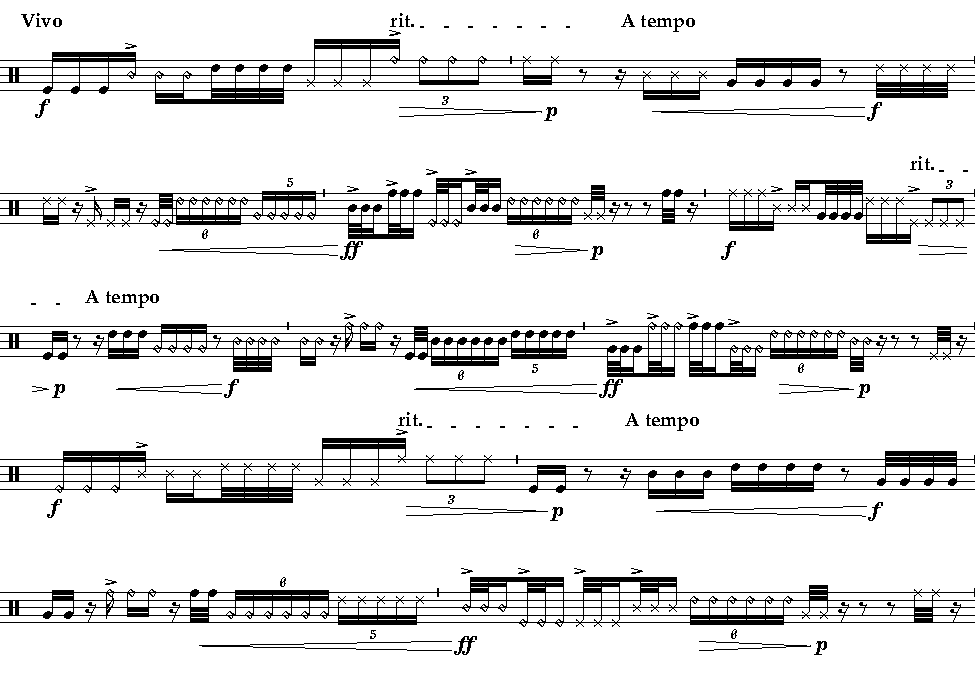
\includegraphics[width=6.5in]{figures/Example_Percussion.pdf}
\caption[Using self-derivation in a percussion setup.]{Using self-derivation to change instruments in a percussion setup.}
\label{fig:percussion}
\end{figure}

%--------------------------------------------------------------------------
Each of the five instruments from each family is notated in Fig.~\ref{fig:percussion} in one of the staff lines, from bottom to top, according to ascending pitch. To discern between the instrument families, tom-toms are notated with a normal note head, cowbells with a diamond, and woodblocks with a cross. The base row $\{0, 2, 3, 1, 4\}$ in Listing~\ref{list:percussion} was chosen specifically not to be retrograde invariant. The set of solutions $\{37, 38, 39, 40\}$, on the other hand, was chosen to fit a particular musical structure. The semi-magic squares in solutions 37 and 38 are the same, and so are the semi-magic squares in solutions 39 and 40. The side vectors in solutions 37 and 38 differ by one row, whereas the side vectors in solutions 39 and 40 differ by two. Moreover, the side vectors in solutions 37 and 38 contain no representatives of the row class contained in the side vectors in solutions 39 and 40, and vice-versa. Therefore the entire passage can be broken into two statements. The motivation for this choice is to make the three repetitions of the basic rhythmic phrase as diverse as possible, avoiding any alignment between the repetitions and the solutions. This is accomplished by the fact that three is relatively prime to four and to two. Dynamics and tempo makings, nevertheless, are aligned with each repeated statement of the rhythmic phrase, since these two musical dimensions belong to the intuitive sphere of this musical composition.

%--------------------------------------------------------------------------
The next musical application is a passage for string quartet where four $4 \times 32$ combination matrices of self-derivation are used to determine pitch. The four instruments are associated with the four rows of the combination matrix in the canonical score order. An 8-tone row is used as the indices of an octatonic scale. The basic index row is $S = \{0, 2, 5, 6, 3, 1, 7, 4\}$. Listing~\ref{list:quartet} displays the output of a modified version of Listing~\ref{writeSolutions} where the base row is $RT_4(S) = \{0, 3, 5, 7, 2, 1, 6, 4\}$. The octatonic row is $\mathcal{O} = \{0, 2, 4, 5, 6, 8, 10, 11\}$, so that $S \mapsto \mathcal{O}$ is the injective mapping

\begin{equation}
	0 \mapsto 0, 1 \mapsto 2, 2 \mapsto 4, 3 \mapsto 5, 4 \mapsto 6, 5 \mapsto 8, 6 \mapsto 10, 7 \mapsto 11 \enspace . 
\end{equation}

%--------------------------------------------------------------------------
\begin{lstlisting}[basicstyle=\ttfamily\footnotesize,numbers=none,caption={Output of Listing~\ref{writeSolutions} for problem size four and row $\{0, 3, 5, 7, 2, 1, 6, 4\}$.},label={list:quartet}]
Solution 86:

     0  3  5  7  2  1  6  4  | 0  3  5  7  2  1  6  4  |
2  |             2           |       5  7              |
28 | 0                 6     |    3        2           | ...
23 |    3  5                 | 0              1  6  4  |
19 |          7     1     4  |                         |

   | 2  5  7  1  4  3  0  6  | 7  1  4  5  2  0  6  3  
   |          1  4  3  0  6  |                         | 62
   |    5  7                 |    1  4                 | 93
   | 2                       | 7                       | 101
   |                         |          5  2  0  6  3  | 106

Solution 116:

     0  3  5  7  2  1  6  4  | 0  3  5  7  2  1  6  4  |
14 |                   6     |    3                    |
30 |             2           | 0     5              4  | ...
19 |          7     1     4  |                         |
0  | 0  3  5                 |          7  2  1  6     |

   | 4  7  1  3  6  5  2  0  | 6  3  1  7  4  5  0  2  
   |                         |       1  7  4  5  0  2  | 50
   |    7  1  3  6           |                         | 67
   |                5  2  0  | 6  3                    | 109
   | 4                       |                         | 125

Solution 161:

     0  3  5  7  2  1  6  4  | 0  3  5  7  2  1  6  4  |
0  |                         | 0  3  5                 |
7  |                         |          7  2        4  | ...
26 |                   6  4  |                1        |
0  | 0  3  5  7  2  1        |                   6     |

   | 7  2  4  6  1  0  5  3  | 0  3  5  7  2  1  6  4  
   | 7  2                    |                1  6  4  | 24
   |          6  1  0  5  3  |                         | 27
   |                         | 0  3  5  7  2           | 85
   |       4                 |                         | 156

Solution 175:

     0  3  5  7  2  1  6  4  | 0  3  5  7  2  1  6  4  |
0  |                         | 0  3  5                 |
9  |                1  6     |                      4  | ...
22 |             2        4  |          7              |
0  | 0  3  5  7              |             2  1  6     |

   | 0  5  3  1  6  7  2  4  | 1  6  4  2  7  0  3  5  
   |                7  2     | 1  6  4                 | 24
   |                         |          2  7  0  3  5  | 85
   | 0  5  3  1  6           |                         | 90
   |                      4  |                         | 140
\end{lstlisting}

%--------------------------------------------------------------------------
\begin{figure}[H]
\centering
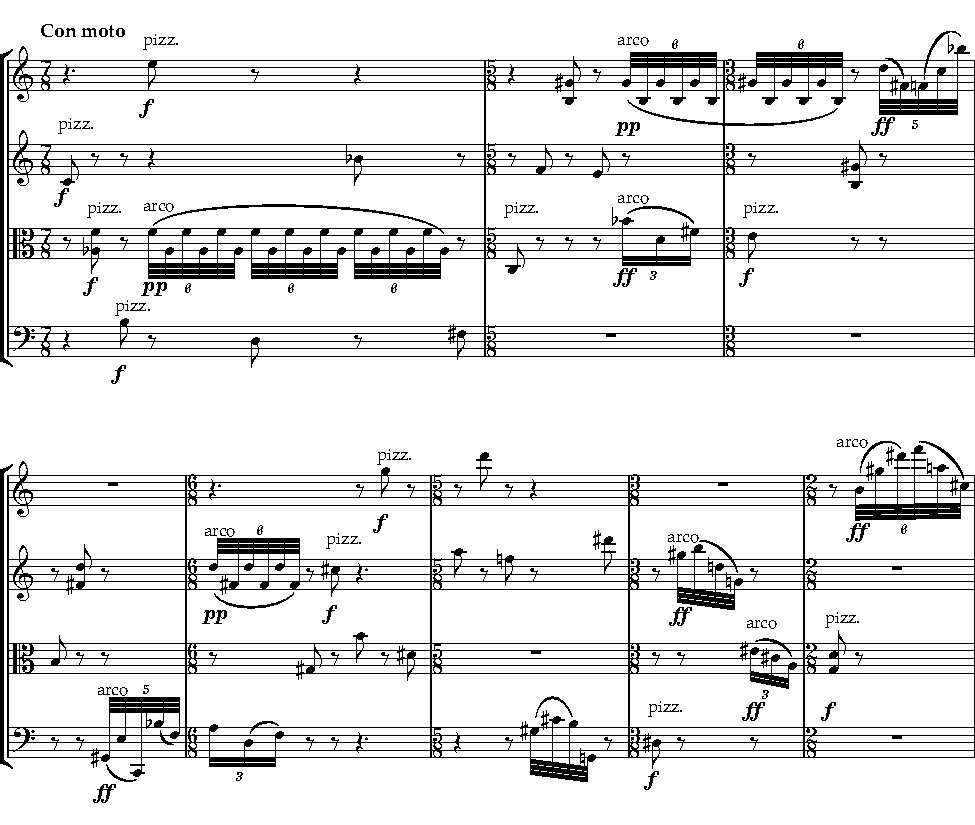
\includegraphics[width=6.5in]{figures/Example_Quartet_1.pdf}
\end{figure}

%--------------------------------------------------------------------------
\begin{figure}[H]
\centering
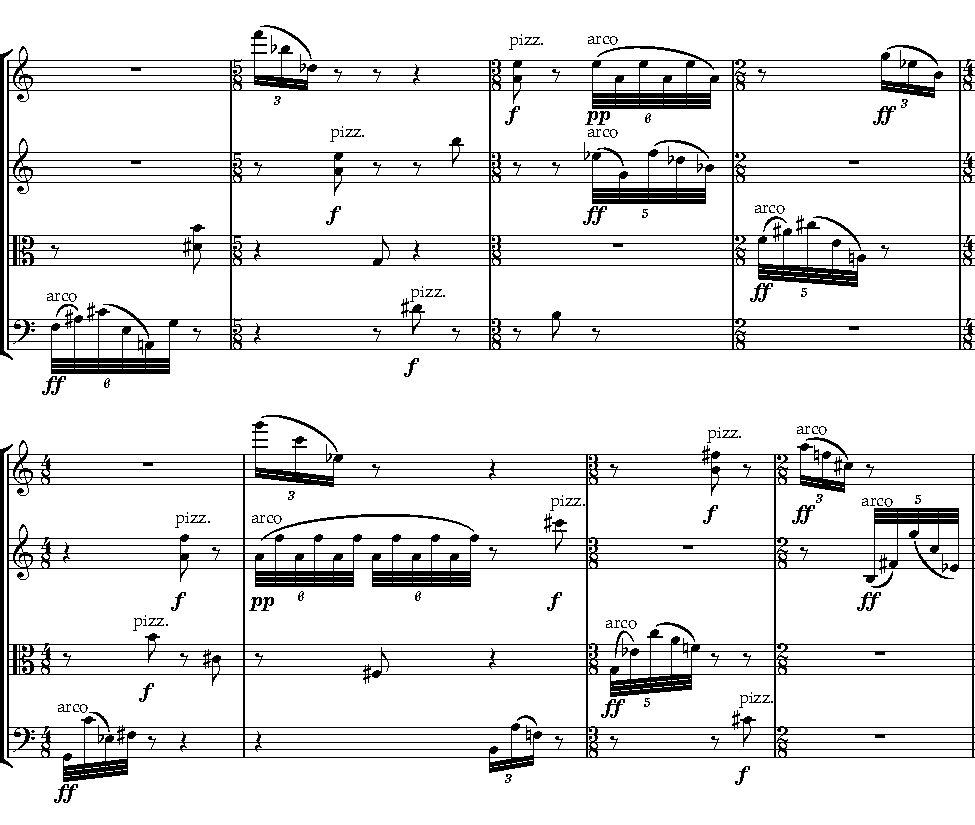
\includegraphics[width=6.5in]{figures/Example_Quartet_2.pdf}
\caption[Using self-derivation with an octatonic scale.]{Using self-derivation to map an octatonic scale to an 8-tone row.}
\label{fig:quartet}
\end{figure}

%--------------------------------------------------------------------------
The output of Listing~\ref{writeSolutions} presented in Listing~\ref{list:quartet} is shown as a musical score in Fig.~\ref{fig:quartet}. The chosen set of solutions is $\{86, 116, 161, 175\}$, and these choices were based mostly on how each semi-magic square explored all instruments. The musical realization is straightforward in regards to how the rows of the combination matrices are mapped to the four instruments. Rhythmically, the contents of the combination matrices are realized depending on the contents of each semi-magic square. Square cells equal to one, two or zero are realized as 8\textsuperscript{th}-notes or rests. Square cells equal to three are realized as 16\textsuperscript{th}-note triplets, cells equal to four are realized as 32\textsuperscript{nd}-notes, and cells equal to five and six are realized as 32\textsuperscript{nd}-note quintuplets and sextuplets, respectively. Cells equal to two are struck simultaneously as double-stops and prolonged as 32\textsuperscript{nd}-note sextuplet tremolos. The tremolo order is the same as the square cell order, and the tremolos have a left and right spacing of one 8\textsuperscript{th}-note, that is, tremolos begin one 8\textsuperscript{th}-note after the double-stop, and end one 8\textsuperscript{th}-note before the next non-empty square cell for that instrument. Tremolos are altogether omitted when there is not enough time for them, hence there needs to be at least three 8\textsuperscript{th}-note rests between a double-stop and the next non-empty cell, so that the tremolo may be surrounded by rests. Besides the tremolos, the remainder of the passage is mostly pointillistic. To emphasize this characteristic, single and double-stop 8\textsuperscript{th}-notes are marked with pizzicati. The time signature changes in this realization are also influenced by the combination matrices. Given the aforementioned durations for each square cell size, every combination matrix column corresponds in Fig.~\ref{fig:quartet} to a bar, such that the time signature of every bar is the sum of the durations of the column cell in the corresponding combination matrix.

%--------------------------------------------------------------------------
\section{Conclusion}

%--------------------------------------------------------------------------
The algorithms, applications and examples presented in this dissertation represent a major advancement in the study of combination matrices of self-derivation. Arguably the most notable contribution is an algorithm that is simple enough to allow computations by hand, while at the same time fast enough to generate thousands of solutions per second when run by a computer, and general enough to compute solutions for arbitrary problem and row sizes. The ideas in \cite{Starr1984} are invaluable for an understanding and classification of various derivation techniques from a set-theoretic perspective. They also contribute enormously to understanding how a particular class of solutions for the self-derivation problem can be constructed by exploring the permutation cycles of $RT_nI$ operations. What is missing in \cite{Starr1984} is an efficient way to compute combination matrices of self-derivation in a general setting. This shortcoming is addressed in \cite{Kowalski1987b}, which restricts its focus to the self-derivation problem and introduces an efficient algorithm to compute solutions for the 12-tone case. Even though the algorithm devised in \cite{Kowalski1987b} can be generalized to other row sizes, it is not a simple algorithm to understand or apply. More importantly, it intentionally avoids computing all possible solutions, sacrificing the less interesting ones for speed. The void that Listing~\ref{allSolutionsRecursive} intends to fill is exactly that of an algorithm that can produce a complete set of solutions given a row and a combination matrix size. The achieved result is straightforward to understand and implement. Devising this algorithm required understanding the problem of self-derivation from a new point-of-view, namely that of a structure that can be broken down into three basic constituent parts: a linearized top, a semi-magic square, and an array of derived row transforms. In this formulation, a top, a square and a side are necessary and sufficient to characterize a solution, that is, every solution is uniquely determined by them according to Th.~\ref{topSquareSideTheorem}. Such analysis of the problem paves the way for a much deeper understanding of self-derivation, especially when combined with a simple and fast algorithm capable of unveiling a large amount of solutions within reasonable time. Once the self-derivation problem was broken into parts, each part had to be studied and understood in detail. This study resulted in reducing the body of solutions into equivalence classes under the action of $RT_nI$, the number and sizes of which depending on the retrograde or retrograde inverse invariance of the row. This body of solutions also groups into classes of solutions which are equivalent under permutations of the side vector, leading to Cor.~\ref{topSquareSideCorollary}, and further into permutations of repeated semi-magic square rows. Although a significant advance, this paper is still a small step toward a more complete understanding of self-derivation, falling short in many aspects. Some of theses aspects will be the subject of the rest of this chapter.

%--------------------------------------------------------------------------
One major weakness of the present implementation is the way tops are pre-computed and stored as binary data. Although this method does improve execution speed, it is impractical, if not impossible, to handle large rows and problem sizes this way, as the number of possible tops becomes quickly unwieldy. One possibility to mitigate this problem would be to compute tops dynamically, compromising execution speed somewhat. In itself, this workaround would not help with the issue that Listing~\ref{allSolutionsRecursive} can produce an unmanageable amount of solutions, many if not most of them being rather uninteresting compositionally. There is a contradiction between a research goal in the present implementation, which is to devise an algorithm that produces a complete body of solutions, and the compositional goal of utilizing combination matrices to achieve meaningful counterpoint. Modifying the current implementation to focus on more interesting combination matrices is very easy, however. Besides the choice of row itself, the main contributor to uninteresting solutions is the semi-magic square itself. Therefore an implementation that restricts the search to squares capable of producing high merge indices should produce highly merged solutions according to the choice of row. Even though the current research is biased toward the understanding of self-derivation in all generality, the methodology described is still suitable for more restrictive applications. Restricting the range of the output of Listing~\ref{allSolutionsRecursive} may also represent a practical way of studying self-derivation itself in cases where the number of solutions is too large. This is an open topic of discussion, however, as what is considered too large is a matter of context. In a distributed system with hundreds of thousands of machines, space requirements and computational times have indeed a completely different meaning. Another argument is that improving how solutions can be further reduced into equivalence classes may involve first being able to produce all solutions. There are several additional ways in which the body of solutions produced by Listing~\ref{allSolutionsRecursive} may be amenable to reduction into representatives of larger and larger equivalence classes. One example is by allowing multiplication, that is, considering the action of the larger group $RT_nMI$. Multiplication in rows of arbitrary size generalizes to studying the group of automorphisms of $\mathbb{Z} / n \mathbb{Z}$, which in turn impacts how row classes are computed and retrograde invariances are filtered. Another example is to allow cyclic rotations of the row. Grouping rows into equivalence classes that include their cyclic rotations is thoroughly described in \cite{FripertingerLackner2015}. The compositional use of combination matrices of self-derivation that include cyclic-rotated transforms of the row can also be seen in \cite{Scotto2000}. Ex.~\ref{ex:scotto} shows how folding a $2 \times 24$ combination matrix of self-derivation into a $4 \times 48$ combination matrix can be achieved by simply repeating the top, that is, extending the top $\{T_0, RT_0\}$ into the top $\{T_0, RT_0, T_0, RT_0\}$. In Ex.~\ref{ex:scotto}, the derived rows contain cyclic-rotated transforms of the original row. Yet another example of how solutions may be reduced is given by how solutions for \emph{different} problem sizes can relate by the technique of folding, whether these relations contemplate cyclic-rotated transforms of the row or not. A particularly interesting consequence of regarding combination matrices of self-derivation as a top, a square and a side is that the set of semi-magic squares have some algebraic structure. It may be possible to reduce the set of solutions produced by Listing~\ref{allSolutionsRecursive} further, but more important could be the potential for generating musical syntax, as any operation that transforms a semi-magic square into another can motivate transforming a combination matrix into another. The action of $RT_nI$ on a combination matrix preserves the semi-magic square, therefore a transformation of the square itself may lead to more interesting musical syntax. Moreover, complete sets of solutions for a problem size and row can also help understanding how these solution sets relate for rows that are generated from the same aggregate realization, as described in \cite{Starr1984}. Comparing sets of solutions, however, brings out a fundamental problem with Listing~\ref{allSolutionsRecursive}, which is the fact that solutions are not output in a standardized order. Given an orbit of solutions under the action of $RT_nI$, a representative for the orbit may be picked by selecting the element where the first derived row is in canonical form. That would ensure that solution sets for different but related rows be more easily compared.

%--------------------------------------------------------------------------
Improving the present implementation may also be considered from the standpoint of execution speed and space requirements. The latter point would involve outputting solutions in a minimized form, such as top, square and side indices. A simple method similar to Listing~\ref{writeSolution} can then be used to reconstruct the solution as a combination matrix. The former point, that is, improving execution speed, is more involved. A simple optimization would be to use SIMD to vectorize vector addition and subtraction, which are fundamental components used in constructing and backtracking semi-magic squares. A more complicated possibility would be to use general purpose computing on the GPU to increase the number of threads. Although possible, this approach brings many complications. The most notable is that GPU programming is very suitable for applications where loops are broken down into into smaller ones and computed by multiple threads that load a single compute kernel. The recursive nature of Listing~\ref{allSolutionsRecursive} goes against this paradigm, and even though recursion is possible on the GPU, it is platform-specific and arguably not the best use of the GPU architecture. In fact, although GPU programming can be platform-independent to an extent, extracting every ounce of performance would likely involve getting into the implementation details of each platform. As mentioned previously, the use of distributed systems can greatly reduce computation times and make space constraints less problematic. It would also require less modifications to Listing~\ref{allSolutionsRecursive}, when compared to the GPU approach. At the same time, the code necessary to distribute the execution of Listing~\ref{allSolutionsRecursive} may be more platform-independent, and not require the modifications necessary to extract compute kernels from Listing~\ref{allSolutionsRecursive} and translate its recursive calls into iterative ones. The difficulty with distributed systems is either the access to a data center, or the cost of building one of a decent size. The use of self-derivation in real-time applications for electroacoustic music represents another area to which the ideas presented here can be extended. In these applications, the current execution speed of Listing~\ref{allSolutionsRecursive} may be adequate and no further optimizations be needed. By nature, combination matrices of self-derivation would fit best within a real-time music application in the sphere of event generation. That may or may not involve MIDI, but the more important observation is that generating events usually occurs at a much slower rate than the digital signal processing of audio samples. The modifications necessary to adapt Listing~\ref{allSolutionsRecursive} to a real-time application might involve not only how many combination matrices are output at a time, but also how these matrices are formatted. One idea is to pair each entry of the top with a timestamp. This vector of timestamps could be algorithmically generated, based on a time-point system, or even triggered by human interaction in live scenarios. Another idea is to pair each entry of each derived row with information regarding their register, if those are being used as pitch classes. Derived rows could also be marked with orchestration information, which in an electroacoustic context could mean the sound source triggered by an element of the derived row, with the derived row itself representing an entire track. For all these example applications, the changes to Listing~\ref{allSolutionsRecursive} would be minimal, and likely only involve adding parameters to it to restrict the output, as well as changing the output to a schematic representation of the combination matrix.

%--------------------------------------------------------------------------
This dissertation explored the concept of self-deriving combination matrices in a general setting. Derivation is a technique that was already used by Schoenberg, in conjunction with hexachordal combinatoriality. The advancements made since Babbitt in the topic of general combinatoriality were reflected on the technique of derivation itself. Although incipient in the work of Martino, Westergaard brings awareness to the possibility of working out by hand $12 \times 144$ combination matrices of self-derivation, and to the fact that more constrained problem sizes are harder to achieve. Starr studies derivation and self-derivation from the standpoint of set theory, formalizing numerous procedures and devising three algorithms. Kowalski subsequently proposes a more general algorithm, focused on the problem of self-derivation. This dissertation expands on the ideas of Starr and Kowalski, proposing a novel algorithm that computes self-deriving combination matrices by separating the problem into a linearized top row, a side vector of self-derived rows, and an underlying semi-magic square. In the process, several mechanisms were devised with the intent to reduce the body of generated solutions into equivalence classes. Examples of the compositional application of self-deriving combination matrices were created to illustrate their use beyond the traditional 12-tone setting. The advancements made in the field of self-derivation are significant, but many directions for future research remain. Understanding how large bodies of solutions relate, both with equal and different problem sizes, such as in folded arrays, is a fundamental way to optimize performance and produce musical syntax.
